\chapter*{Problema}
\label{cha_problema}

Il problema del commesso viaggiatore consiste nella ricerca del ciclo hamiltoniano più breve all'interno di un grafo pesato completo. Questo tipo di problema appartiene alla classe dei problemi \emph{NP-Completi}. In Figura~\ref{fig_eil76} è mostrato uno dei problemi TSP con soluzione, sottoinsieme dei problemi NP.

\begin{figure}
  \centering
  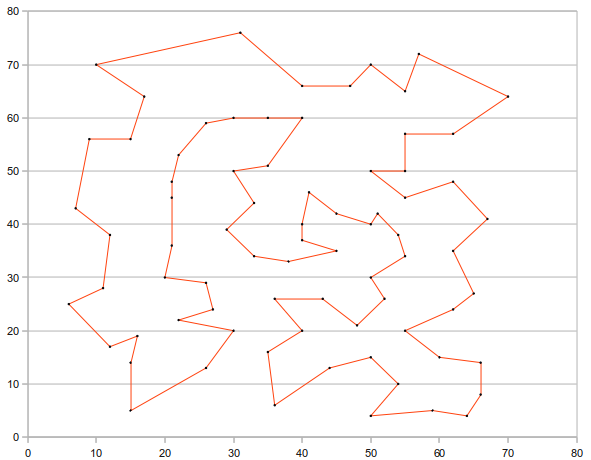
\includegraphics[width=10.0cm]{immagini/eil76.png}
  \caption{Eil76, problema di TSP da 76 città\label{fig_eil76}}
\end{figure}

Il compito assegnato è di generare una soluzione ammissibile e quanto più possibile vicina a quella ottimale (ovvero la migliore) in 3 minuti di esecuzione del programma. Il programma deve poter lavorare su 10 problemi diversi:
\begin{itemize}
  \item \emph{ch130};
  \item \emph{d198};
  \item \emph{eil76};
  \item \emph{fl1577};
  \item \emph{kroA100};
  \item \emph{lin318};
  \item \emph{pcb442};
  \item \emph{pr439};
  \item \emph{rat783};
  \item \emph{u1060}.
\end{itemize}

